\normaltrue \difficilefalse \tdifficilefalse
\correctiontrue

%\UPSTIidClasse{11} % 11 sup, 12 spé
%\newcommand{\UPSTIidClasse}{12}

\exer{Système vis-écrou $\star$ \label{C2:06:36}}
\textit{D'après ressources Pole Chateaubriand -- Joliot-Curie.}
\setcounter{question}{0}\UPSTIcompetence[2]{A3-05}
\UPSTIcompetence[2]{C2-06}
\index{Compétence C2-06}
%\index{Train d'engrenages simple}
\ifcorrection
\else
\marginnote{\textbf{Pas de corrigé pour cet exercice.}}
\fi

\ifprof
\else
Soit la chaîne de transmission suivante. 
\begin{center}
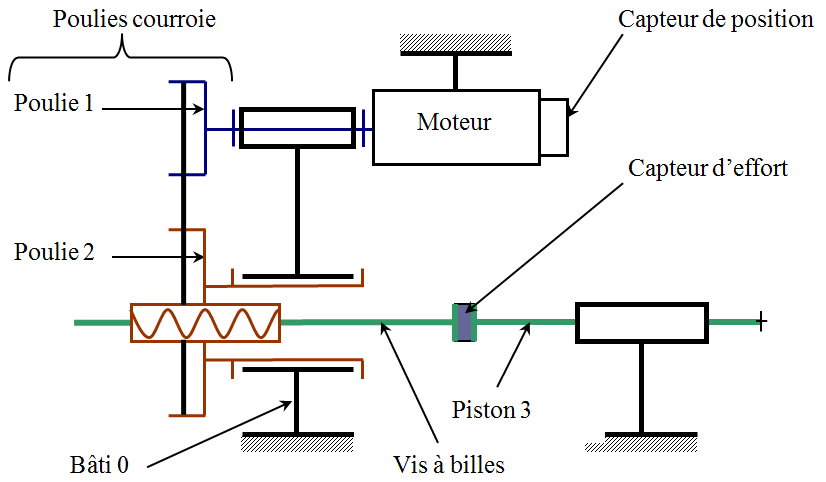
\includegraphics[width=\linewidth]{36_01}
\end{center}

Le schéma du restituteur actif est donné ci-dessous. Le pas de la vis est $p_v =\SI{10}{mm}$.
Le diamètre de la poulie 2 est le double de celui de la poulie 1. 


\fi


\question{Sur le schéma cinématique, repasser chaque solide d’une couleur différente.}
\ifprof
\else
\fi

\question{Réaliser la chaîne d’énergie-puissance partielle en définissant les noms des transmetteurs et les grandeurs
d’entrée et de sortie cinématiques.}
\ifprof ~\\
\else
\fi

\question{Définir la loi entrée-sortie entre la vitesse de translation du piston 3 et la vitesse de rotation du moteur~1. }
\ifprof~\\
%On a $Z_3 = 2Z_2 + Z_1$.
\else
\fi

\ifprof
\else
\begin{flushright}
\footnotesize{Corrigé  voir \ref{C2:06:36}.}
\end{flushright}%
\fi